
%%%%%%%%%%%%%%%%%%%%%%% file typeinst.tex %%%%%%%%%%%%%%%%%%%%%%%%%
%
% This is the LaTeX source for the instructions to authors using
% the LaTeX document class 'llncs.cls' for contributions to
% the Lecture Notes in Computer Sciences series.
% http://www.springer.com/lncs       Springer Heidelberg 2006/05/04
%
% It may be used as a template for your own input - copy it
% to a new file with a new name and use it as the basis
% for your article.
%
% NB: the document class 'llncs' has its own and detailed documentation, see
% ftp://ftp.springer.de/data/pubftp/pub/tex/latex/llncs/latex2e/llncsdoc.pdf
%
%%%%%%%%%%%%%%%%%%%%%%%%%%%%%%%%%%%%%%%%%%%%%%%%%%%%%%%%%%%%%%%%%%%


\documentclass[runningheads,a4paper]{llncs}

\usepackage{amssymb}
\setcounter{tocdepth}{3}
\usepackage{graphicx}
\usepackage{float}
\usepackage[full]{complexity}
\usepackage{amsmath}
%\usepackage{amsfonts}
%\usepackage{amsthm}
\usepackage{subfigure}
%\usepackage{caption}
%\usepackage{subcaption}
%\usepackage{cite}
\usepackage{hyperref}
\usepackage{url}
\usepackage{clrscode4e}
\urlstyle{same}
\newcommand{\keywords}[1]{\par\addvspace\baselineskip
\noindent\keywordname\enspace\ignorespaces#1}

% Uniform numbering for previously defined theorem environments (e.g., LNCS).
\makeatletter
\let\c@lemma=\c@theorem
\let\c@corollary=\c@theorem
\let\c@fact=\c@theorem
\makeatother

% Redefinition of LNCS or SODA or Springer proof environment to put a \Box at
% the end of every proof.
\let\realendproof=\endproof
\def\endproof{\hspace*{\fill}$\Box$\realendproof}


\begin{document}

\mainmatter  % start of an individual contribution

% first the title is needed
\title{The Complexity of Designing the Hardest Instances}

% a short form should be given in case it is too long for the running head
\titlerunning{The Complexity of Designing the Hardest Instances}

% the name(s) of the author(s) follow(s) next
%
% NB: Chinese authors should write their first names(s) in front of
% their surnames. This ensures that the names appear correctly in
% the running heads and the author index.
%
\author{Fermi Ma \and Ariel Schvartzman \and Erik Waingarten}
%
\authorrunning{Fermi Ma \and Ariel Schvartzman \and Erik Waingarten}
% (feature abused for this document to repeat the title also on left hand pages)

% the affiliations are given next; don't give your e-mail address
% unless you accept that it will be published
\institute{MIT,\\
77 Mass Ave., Cambridge, MA 02139, USA, \\
\protect\url{{fermima,arielsc,eaw}@mit.edu}}

%
% NB: a more complex sample for affiliations and the mapping to the
% corresponding authors can be found in the file "llncs.dem"
% (search for the string "\mainmatter" where a contribution starts).
% "llncs.dem" accompanies the document class "llncs.cls".
%

\maketitle

\section{Introduction}

In 2012, McGuire, Tugemann, Civario confirmed the conjecture that there is no 16-clue Sudoku puzzle \cite{mcguire2012there}. The graduate students in MIT's Math Department were so surprised by this result that there is a copy of the arXiv preprint on a wall on the 4th floor of the department, next to the lounge. The paper described novel techniques to enumerate through all the possible 16-clue puzzles, and the computation lasted from January 2011 to December 2011. 

We are interested in formalizing this question for other puzzles. Consider the following scenario. There are two parties: a puzzle maker $M$ and a puzzle solver $S$. $M$ wants to design the hardest puzzles for $S$ to solve. $S$ reads the puzzles on the newspaper, so $M$ must make sure to provide the solution along with the puzzle. 

Most algorithmic results in this field ask how hard it is for $S$ to solve a puzzle. We are interested in the other side of the question: how hard is it for $M$ to design the hardest puzzle. By hardest, we mean the least number of clues. For example, for a Sudoku, we mean the least number of given entries. We also want to disallow certain cases. For instance, $M$ obviously would not publish the empty Sudoku puzzle since the solution he provides might be different from how $S$ solves it. We will only look at puzzles with clues such that the solution is \emph{unique}.

In this paper, we are interested in determining how hard it is to compute hardest instances for the case of Sudoku. For that purpose, we will introduce an appropriate framework and define a complexity class, called $\mathsf{SPC}$. We will then present the problems that are essential to understanding the complexity of Sudoku. These c well known problems such as SAT and 3SAT, as well as other puzzles such as Latin Squares. After introducing these problems, we will show that they are all complete in the $\mathsf{SPC}$ class using known reductions. We conclude by providing upper bounds on the $\mathsf{SPC}$ class and posing interesting open questions. 

In Section~\ref{sec:prelim}, we define the complexity class $\mathsf{SPC}$, relate it to the problem we are trying to solve and provide lower bounds for the class by showing it contains common complexity classes. In Section ~\ref{sec:The Problems} we formalize the problems that will help us understand the complexity of Sudoku in this class. These were mentioned above. Then in Section~\ref{sec:complete}, we exhibit a chain of reductions to show the problems in Section~\ref{sec:The Problems} are complete for this class. Finally, we conclude with some thoughts and open problems.

\textbf{Related Work} Insert related work here. 

\section{Preliminaries}
\label{sec:prelim}

\begin{definition}
We will call a puzzle \emph{valid} if it has a unique solution.
\end{definition}

In general, we assume that $M$ has the following workflow:
\begin{enumerate}
\item $M$ decides which kind of puzzle.
\item $M$ decides how "big" the puzzle will be.
\item $M$ wants to induce some deductive response by $S$, so it designs small parts of the puzzle.
\item $M$ must make sure that the puzzle is valid, by adding the smallest number of additional clues.
\item $M$ computes the solution and publishes it. 
\end{enumerate}

We can define the problem of \emph{computing the hardest instances} in the following way: 

\begin{quote}
Given a problem with a polynomially sized solutions, what is the minimum number of clues we must give in order for the problem to contain the clues in the solution, and for there to be a unique solution?
\end{quote}

We will ask the decision version of the problem: does there exist a set of at most $k$ clues which give rise to a unique solution?

We now define terms which will be related to the "minimum clues" problem for puzzles. These definitions will give rise to a complexity class, which we call  $\mathsf{SPC}$ (for Smallest Partial Certificate). We can assume without loss of generality that non-deterministic Turing machines (NTMs) have a branching factor of $2$ at each non-deterministic step. In addition, we assume that we have a canonical ordering of the two branches, so we can call one the "left" branch, and the other the "right" branch. We also assume without loss of generality that all branches of the computation have length equal to a fixed polynomial.

\begin{definition}
A partial certificate is a read-only tape which contains at each tape cell one of three possible characters, 0, 1, or \emph{blank}, which we denote as $\bot$.
\end{definition}

\begin{definition}
The size of a partial certificate is the number of non-null entries. 
\end{definition}

For problems in $\NP$, a partial certificate is the generalization of a certificate of an $\NP$ problem. Each certificate of an $\NP$ problem is a partial certificate. We can think of partial certificates as a certificate, where we erase some tape cells.

\begin{definition}
A modified non-deterministic Turing machine (mNTM) is a NTM where there is an additional input of a partial certificate. At each step of the computation, a mNTM reads the next tape cell of the partial certificate and if the partial certificate contains a 0, it takes the left branch of the computation. If it contains a 1, it takes the right branch of the computation. If it contains $\bot$, then it behaves non-deterministically. Other than that, an mNTM behaves exactly like an NTM.
\end{definition}

In some sense, a partial certificate makes a mNTM more deterministic. If a partial certificate contains no $\bot$, then the mNTM behaves like a deterministic Turing machine. Alternatively, we can think of the partial certificate as feeding in clues to the mNTM in order to guide its computation. We say that a NTM has a corresponding mNTM which runs exactly the same, but has an additional input for a partial certificate. With these definitions, we are ready to define the class $\mathsf{SPC}$.

\begin{definition}
$\mathsf{SPC}$ is the class of decision problems of the following form:\\
\begin{quote}
Given a NTM running in polynomial time and a parameter $k$, does there exists a partial certificate of size at most $k$ such that the corresponding mNTM with the partial certificate has only one accepting branch?
\end{quote}
\end{definition}

\begin{proposition}
Any problem of determining the smallest number of clues is in $\mathsf{SPC}$, and alternative, any problem in $\mathsf{SPC}$ can be phrased as a problem to determine the smallest number of clues.
\end{proposition}

\begin{proof}
Our problems have polynomially long solutions, which can be checked in polynomial time. Therefore, we can create the NTM that non-deterministically generates a solution, and checks whether the solution works deterministically. Computing the if this NTM has a partial certificate of size at most $k$ with only one accepting branch is equivalent to asking whether there exists $k$ clues which give rise to a unique solution. 

Alternatively, if we have a NTM running in polynomial time, then we can think of the problem as finding which turns at the branches one must take in order for the NTM to accept. A partial certificate of size at most $k$ is equivalent to $k$ clues which give rise to a unique solution.
\end{proof}

The above proposition justifies our analysis of this class for answering these questions.

\subsection{Relation to known complexity classes.}

Here we present lower bounds for the complexity class $\mathsf{SPC}$. It remains to be shown if any of the containments is strict. It is the opinion of the authors that this is likely to be true. 

\begin{proposition}
If a problem is $\mathsf{SPC}$-hard, then it is $\NP$-hard.
\end{proposition}

\begin{proof}
If a problem is in $\NP$, then there exists a NTM which decides in time at most $p(n)$, where $p$ is a polynomial and $n$ is the size of the input. We can ask if there exists a partial certificate of size at most $p(n)$? Therefore, $\NP \subset \mathsf{SPC}$, and so any $\mathsf{SPC}$-hard problem is also $\NP$-hard. 
\end{proof}

\begin{proposition}
If a problem is $\mathsf{SPC}$-hard, then it is $\coNP$-hard. 
\end{proposition}

\begin{proof}
$\mathsf{UNIQUE-SAT}$ is in $\mathsf{SPC}$ since we can ask whether there is a partial certificate of size at most $0$. This implies that $\coNP \subset \mathsf{US} \subset \mathsf{SPC}$ since UNIQUE-SAT is complete in $\mathsf{US}$ \cite{blass1982unique}.
\end{proof}

\section{The Problems}
\label{sec:The Problems}

We present a formalism of the type of problems we wish to solve. Each problem will be defined with an \emph{instance} of the problem which will be an encoding of the problem into a string of polynomial size, along with a value $k$. The resulting output will be a decision signifying there exists $k$ clues which will solve the instance uniquely. This framework will fit in nicely with the problems we are trying to solve.

The basic premise is that a puzzle maker wants to induce some kind of particular deduction in the puzzle solver. The puzzle maker begins designing the puzzle, which becomes the instance to the problem. Additionally, the puzzle maker asks how many clues it must add, it does so by specifying a value $k$, and asking whether there are at most $k$ clues which will lead to a valid puzzle.

\subsection{$\mathsf{SPC-Sudoku}$}

We first introduce the problem which motivated this study. In Sudoku puzzles, we are given a $n^2 \times n^2$ grid consisting of $n^2$ $n \times n$ bolded blocks, some of whose entries have been filled in with number from $1$ to $n^2$. Often in the literature, $n$ is referred to as the order of the puzzle. The goal of the game is to fill in the rest of the grid with numbers from $1$ to $n^2$ while enforcing that no row, column or bolded square repeats a numbers. 

\begin{itemize}
\item Instance: A partially filled Sudoku puzzle, along with a parameter $k$.
\item Question: Does there exists at most $k$ clues which will yield a valid Sudoku puzzle?
\end{itemize}

Note that when the instance is an empty Sudoku puzzle of order 3, the question becomes exactly the question of determining the size of the valid Sudoku puzzles. This particular instance of our problem can easily solve the problem that \cite{mcguire2012there} computed. 

\subsection{$\mathsf{SPC-LatinSquares}$}

n Latin Squares, we are given a $n \times n$ grid, some of whose entries have been filled in with numbers from $1$ to $n$. The goal of the game is to fill the rest of the grid with numbers from $1$ to $n$ while enforcing that no row or column repeats a number. 

In fact, it is know that each such square gives rise to a \emph{quasi-group}. The problem of Latin Squares asks whether a partially filled Latin Square can be completed. It is known that such problem is \NP-complete. We present the problem $\mathsf{SPC-Latin Squares}$ in our framework.

\begin{itemize}
\item Instance: A partially filled latin square, along with a parameter $k$. 
\item Question: Does there exists at most $k$ clues which will yield a valid Latin Squares puzzle?
\end{itemize}

\subsection{$\mathsf{SPC-Triangle Partition}$}

This problem is a known $\NP$-complete problem which asks to partition the edges of a graph into triangles \cite{holyer1981np}. We present the ``minimum clues" version of the problem since we will use it to show hardness results for $\mathsf{SPC-Latin Squares}$ and $\mathsf{SPC-Sudoku}$. There is a general description of the problem in \cite{holyer1981np}. A specific instance is addressed in \cite{colbourn1984complexity}. We will use the definition in \cite{colbourn1984complexity}. We first present a definition of a property of tripartite graphs which will simplify the analysis.

\begin{definition}
A tripartite graph is \emph{uniform} if each vertex has equally many neighbors in each of the other two partitions.
\end{definition}

\begin{itemize}
\item Instance: A uniform tripartite graph, along with a parameter $k$.
\item Question: Does there exists at most $k$ triangles which give rise to a unique partition of the graph into triangles?
\end{itemize}

Note that if a tripartite graph has a triangle partition, the graph must be uniform, so even though the requirement that the graph be uniform is not necessary, it simplifies the analysis.

\subsection{$\mathsf{SPC-SAT}$}
The following is the obvious generalization for giving clues in the Boolean satisfiability problem.

\begin{itemize}
\item Instance: a Boolean formula $\phi$, along with a parameter $k$.
\item Question: Is there an assignment of at most $k$ variables where the corresponding Boolean formula is satisfied uniquely?
\end{itemize}

\section{Complete Problems}
\label{sec:complete}

In this section, we proceed to show that $\mathsf{SPC-Sudoku}$ is $\mathsf{SPC}$-complete. In order to do so, we first show that $\mathsf{SPC-SAT}$ is $\mathsf{SPC}$-complete. We then follow a known chain of reductions that is used to show that the problem of filling in a Sudoku is $\mathsf{NP}$-complete. 

It is important to note at this point that in order for a problem to be $\mathsf{SPC}$-complete, it needs to belong to the class as well as be reducible to any other problem in the class. In this context, we use the classical Karp single-call notion of a reduction. 

\begin{theorem}
$\mathsf{SPC-SAT}$ is $\mathsf{SPC}$-complete.
\end{theorem}

\begin{proof}
The proof is similar to the Cook-Levin theorem. We use the proof in \cite{Garey}. We can first turn an arbitrary NTM into an NTM with a bigger alphabet where at each step, if the NTM in state $q$ writes $a$ into some tape cell, then the other NTM writes $(q,a)$ into the same tape cell. Once we have this, we apply the reduction from the Cook-Levin theorem, to get a Boolean formula $\phi$. 

We claim that if $\phi$ has a partial assignment of $k$ variables with a unique complete assignment, then there exists a partial certificate for the NTM with corresponding mNTM having only one accepting branch of the computation.

Note that if a partial assignment of $k$ variables contains a variable that is set to false, then the variable is a head position variable, a state variable, or a tape cell variable. We know that there exists a head position variable, a state variable, and a tape cell variable which is true at each time, so if we switch the corresponding variables, we have removed a false variable, added a true variable, and by analyzing $\phi$, the true variable implies that the false variable is false, therefore, we still have a partial certificate. 

Therefore, we can assume that all assignments are true. If we have a head position variable, the tape cell variable at that given position will be set to true, and so switching them will maintain the partial assignment. Also, since the content of each tape cell is the state-content tuple, a state variable can be replaced by the tape cell variable. Therefore, we can assume that we have a partial assignment of the tape-cell variables, which are all true. 

Since each complete assignment of the variables corresponds to a unique accepting branch of the computation, knowing the contents of the tape cell at each time tells you which branch of the computation to take. Therefore, if there exists a partial assignment of $k$ variables which yield a unique complete assignment, then there exists a partial certificate of size $k$ whose mNTM has a unique accepting branch.
\end{proof}

From this we can easily show that the corresponding $3SAT$ problem is $\mathsf{SPC}$-complete. We follow the reduction 

\begin{theorem}
$\mathsf{SPC-3SAT}$ is $\mathsf{SPC}$-complete.
\end{theorem}

\begin{proof}
We reduce from $\mathsf{SPC}$-SAT and apply the parsimonious reduction of \cite{yaleclass}. We can assume without loss of generality that the SAT formula is a conjuction of clauses, which are disjunctions, since these are the formulas for the Cook-Levin theorem. Suppose that we have a set of clauses $\{ C_i \}$, then transform the clauses by succesively applying the following function $g$ to each clause $C = (x_1 \vee x_2 \vee ... \vee x_k)$:
\[ g(C) = \left\{ \begin{array}{cc} C & k \leq 3 \\
						    (z_1 \vee x_1 \vee x_2) \wedge (\overline{z_1} \vee \overline{x_1}) \wedge (\overline{z_1} \vee \overline{x_2}) \wedge (\overline{z_1} \vee x_3 \vee ... \vee x_k) & \text{ otherwise }\end{array} \right. \] 

Suppose $z_i$ is in a partial certificate of 3SAT. There are two cases:
\begin{itemize}
\item $z_i$ is set to false. In this case, we know that either $x_1$ or $x_2$ is set to true. If we switch $z_i$ and $x_1$ or $x_2$, one of these will be partial certificate which is the same size as the previous one, since the value of $z_i$ is implied by one of $x_1$ or $x_2$. Therefore, we can include $x_1$ or $x_2$ and remove $z$.
\item $z_i$ is set to true. Then $\overline{z_i}$ is false, which means that whichever $\overline{z_i}$ ends up being a part of in the clause will mean that one of two of the following will be true. Again, if we switch them, one will have a smallest partial certificate which is of the same size. So we can remove $z_i$ and replace it by another variable. 
\end{itemize}
Note that in the above procedure, we maintained the size of the partial certificate, and either removed $z_i$ and added a variable which was in SAT, or replaced it by $z_{i+1}$. Since there are a limited number of $z_i$, we can repeat this procedure and arrive at a partial assignment of the 3SAT formula which works for the SAT formula as well.
\end{proof}

The following proof is a sketch and is under revision.

\begin{theorem}
$\mathsf{SPC-Triangle Partition}$ is $\mathsf{SPC}$-complete.
\end{theorem}

\begin{proof}
We use the reduction from \cite{holyer1981np}, applying the slight modifications made in \cite{colbourn1984complexity} so that the graph is tripartite. 

Note that in the reduction, if one has $k$ triangles and one of the triangles belongs to a join, then that triangle is implied by a neighboring triangle. So we can assume that all triangles are either in $H_{3,p}$ of variables, or $H_{3,p}$ of literals. 

In addition, if one of the $k$ triangles is a $T$-patch triangle in an $H_{3,p}$ of a literal, then there exists a triangle in an $F$-patch of another literal, so can switch them.

So in $k$ triangles, we can either assume they are in an $H_{3,p}$ of a variable, or an $H_{3,p}$ of a false literal. So if there is a partition of $k$ triangles which makes a unique edge partition, then there exists an assignment of $k$ variables which uniquely determine the assignment of all the variables to satisfy the formula. 

Likewise, if there is an assignment of $k$ variables, then in each clause, there is at least one variable which satisfies the clause. So we can switch the triangle in the variable, for the triangle in the clause which satisfies it. This implies the variable, so we can do this.
\end{proof}

\begin{theorem}
$\mathsf{SPC-Latin Squares}$ is $\mathsf{SPC}$-complete.
\end{theorem}

\begin{proof}
We do this via reduction from the triangle partition problem. Given a tripartite graph $G$, we first check whether or not it is uniform. If it is not uniform, then there does not exist a triangle partition. If it is uniform, we can write down a latin framework $LF(G;2n,2n,2n)$ in polynomial time (cite...). Since the Latin framework is constructed so that $G$ is a defect of $LF(G;2n,2n,2n)$, there is a triangle partition of $G$ if and only if we can complete the partial latin square $LF(G;2n,2n,2n)$. This completes the proof.

We claim that the above proofs can give us an $\mathsf{SPC}$-hardness result for completing a partial Latin square. To see this, note that the triangle partitions of a defect graph $G(P)$ are in one to one correspondence with the solutions to the Latin square $P$.
\end{proof}

\begin{theorem}
$\mathsf{SPC-Sudoku}$ is $\mathsf{SPC}$-complete
\end{theorem}

We will show the proof from \cite{takayuki2003complexity}. For proofs of the following two propositions, refer to the paper. 

\begin{proposition}
Let $S_0$ be defined as
$$S_0 (i,j) = ((i \mod n) n + \lfloor i/n \rfloor + j) \mod n^2. $$
Then $S_0$ represents a solution to an order $n$ Number Place. 
\end{proposition}

\begin{proposition}
Let $S$ be a Number Place puzzle of order $n$ such that
\begin{displaymath}
S(i,j) = \left\{
\begin{array}{lr}
\perp & : (i,j) \in B\\
S_0 (i,j) & : \text{otherwise}
\end{array}
\right.
\end{displaymath}

where $B = \{ (i,j) | i < n \text{ and } (j \equiv 0) \mod n \}$. Then a square $S'$ obtained by filling in the blanks of $S$ is a solution to $S$ if and only if

\begin{itemize}
\item For any $(i,j) \in B$, $S'(i,j) \equiv 0 \mod n$
\item A square $L$ defined by $L(i, j/n) = S'(i,j)/n$ for all $(i, j) \in B$ is a Latin Square.
\end{itemize}

\end{proposition}

\begin{proof} 

We will show an $\mathsf{SPC}$ reduction from $\mathsf{SPC-Latin Squares}$ and argue that it can be done in polynomial time.

Suppose we are given a Latin Square $L$ of order $n$. We will construct a Sudoku instance of order $n$ as follows:
\begin{displaymath}
S(i,j) = \left\{
\begin{array}{lr}
\perp & : (i,j) \in B, L(i, j/n) = \perp \\
L(i, j/n) n & : (i,j) \in B, L(i, j/n) \neq \perp \\
S_0 (i,j) & : \text{otherwise}
\end{array}
\right.
\end{displaymath}
This construction can be done in polynomial time. In addition, from our previous analysis we know that any solution of $L$ has a unique corresponding solution of $S$. Therefore, we get a polynomial time $\mathsf{SPC}$ reduction.

\begin{figure}[H]
\label{fig:partialLS}
\centering
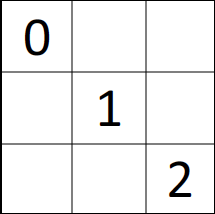
\includegraphics[scale=0.25]{sudoku-3.png}
\caption{Example of partial Latin Square of order 3.}
\end{figure}

\begin{figure}[H]
\label{fig:partialNP}
\centering
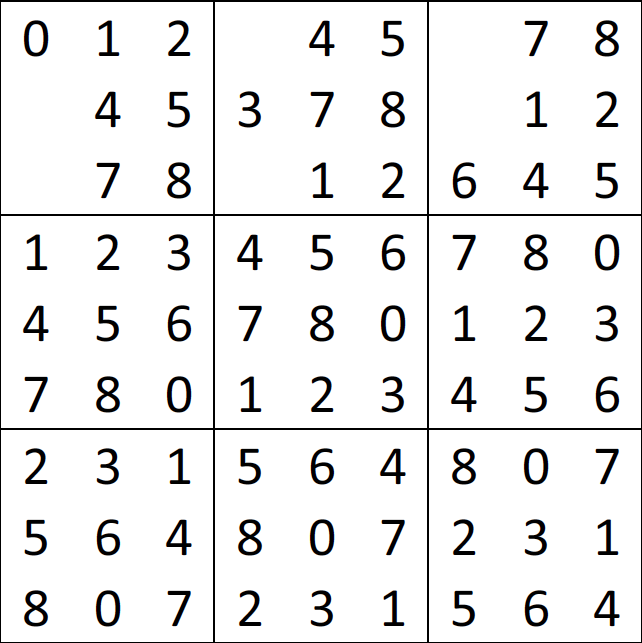
\includegraphics[scale=0.25]{sudoku-1.png}
\caption{Example of corresponding partial Number Place on a board of order 3.}
\end{figure}

\end{proof}

\subsection{Upper Bounds}

We provide an algorithm for solving $\mathsf{SPC-SAT}$ with an NTM with a SAT oracle. This will mean that $\mathsf{SPC} \subset \NP^{\NP}$ and so the complete problems will probably not be $\PSPACE$-hard. If an $\mathsf{SPC}$-complete problem were $\PSPACE$-hard, it would collapse most of the polynomial time hierarchy \cite{stockmeyer1976polynomial}. 

\begin{lemma}
A Boolean formula $\phi$ has a partial assignment of $k$ variables which yield a unique solution if and only if every variable outside the partial assignment, one assignment yields a satisfiable formula, and one does not.
\end{lemma}

\begin{proof}
This is clear since there is only one accepting branch.
\end{proof}

\begin{lemma}
A Boolean formula $\phi$ has no partial assignment of $k$ variables if and only if there exists an additional variable which both assignments give a satisfiable Boolean formula.
\end{lemma}

\begin{proof}
If there are at least two accepting branches of the computation. Compute the least common ancestor of the branches in the computation tree. That will yield a variable which can take on both assignments. 
\end{proof}

\begin{codebox}
\Procname{$\mathsf{SPC-SAT}$: Instance: $\phi$ formula with variables $\{ x_i \}$ and variable $k$.}
\li \For $i = 1, ..., k$ \Then
\li Non-deterministically pick a variable $x_i$, without repetition
\li Non-deterministically pick an assignment \End
\li Iterate through all remaining variables \Then
\li \If a variable has both assignments with a satisfiable boolean formula \Then
\li reject
\li \Else assign that variable \End \End
\li Once you assigned all variables, accept.
\end{codebox}

\begin{proposition}
$\mathsf{SPC} \subset \NP^\NP$
\end{proposition}

\begin{proof}
Use the above algorithm to solve $\mathsf{SPC-SAT}$. 
\end{proof}

\section{Conclusion}

We have formalized the notion of what it means to compute the hardest instance to a puzzle by providing the minimum clues. This gave rise to $\mathsf{SPC}$, and we showed some problems were complete for this class. In particular, this means $\mathsf{SPC-Sudoku}$ is $\NP$-hard, but is unlikely to be $\PSPACE$-hard. However, the instances of $\mathsf{SPC-Sudoku}$ which make it $\mathsf{SPC}$-complete are very far from empty. In fact, just by looking at the last reduction from $\mathsf{SPC-Latin Squares}$, a Sudoku of dimensions $n^2 \times n^2$ which is a hard instance, at most $n^2$ of the $n^4$ squares at empty. It would be interesting to see if the empty instances of Sudoku are still complete for $\mathsf{SPC}$. This would be exactly the problem \cite{mcguire2012there} solved for $n = 3$. 

\bibliography{references}
\bibliographystyle{splncs}
\end{document}
